\documentclass[12pt,a4paper,titlepage]{article}

\usepackage[utf8]{inputenc}
\usepackage{amsmath}
\listfiles
\usepackage[T1]{fontenc,url}
\usepackage[firstinits=false,url=false,isbn=false,style=authoryear,backend=biber,sorting=nyt,maxcitenames=2,uniquelist=false,maxbibnames=12,
uniquename=false,texencoding=utf8,bibencoding=utf8]{biblatex}
\renewcommand*{\finalnamedelim}{\addspace\&\space}
\addbibresource{ScottRef.bib}
\usepackage{etoolbox}
\usepackage{keyval}
\usepackage{import}
%\usepackage{fancyhdr}
%\pagestyle{fancy}
%if biber broken, run <rm -rf `biber --cache`> in terminal

\usepackage{csquotes}
\usepackage[american]{babel}
\usepackage{verbatim}
\makeatletter
\patchcmd{\Ginclude@eps}{"#1"}{#1}{}{}
\makeatother
\usepackage[margin=1in]{geometry}
\usepackage{array,booktabs}
\usepackage{ifdraft}
\geometry{a4paper}
\usepackage{graphicx}
\usepackage{import}
\usepackage{latexsym}
\usepackage{grffile}
\usepackage[nolists]{endfloat}

\usepackage{tabularx}
%\usepackage{figcaps}
%\usepackage{dontdistribute}
%\usepackage{draftdatetime}
\usepackage[hang,flushmargin]{footmisc}
\renewcommand{\thesection}{\arabic{section}}

\usepackage{setspace}


\let\oldtabular\tabular
\renewcommand{\tabular}{\footnotesize\oldtabular}
\DeclareUnicodeCharacter{00A0}{ }
\DeclareUnicodeCharacter{202D}{}
\DeclareUnicodeCharacter{202C}{}


\title{Analyzing policy networks using valued exponential random graph models (ERGMs): To what extent do government-sponsored collaborative groups enhance organizational networks?}
%\author{Tyler Scott\\ Evans School of Public Affairs, University of Washington}
%\date{June 2014}



\begin{document}

\singlespacing
\maketitle

\begin{abstract}
\singlespacing

This paper examines collaborative management groups from the perspective of policymakers seeking to increase coordination amongst organizations within a policy network. of the sponsoring agency. While governments often initiate and support collaborative groups as a tool to address perceived network failures such as a lack of coordination, the net impact groups have is unclear. To address this question, I use valued exponential random graph models (ERGMs) to model relationships of varying strength amongst a regional network of organizations involved in 57 collaborative groups. This provides a unique opportunity to study the interplay between numerous groups and organizations within a large-scale network. Valued ERGMs are a recently developed extension of standard ERGMs that model binary ties; thus, this paper makes also makes a methodological contribution to the policy literature. Findings suggest that participation in collaborative groups does motivate increased network ties between individual organizations; this effect is strongest for: (a) organizations that are not already members of another group; and (b) groups minimize membership overlap with other groups. These results support a transaction-cost based perspective of how collaborative groups can influence organizations within a network to initiate and maintain cooperative ties with one another.\\



\noindent
\bf{Keywords}: Collaborative management, policy networks, ERGM, valued ties, network analysis, transaction costs
\end{abstract}

\doublespacing
%\keywords{collaborative management, policy networks, ERGM, network analysis}
\section{\bf\MakeUppercase{Introduction}}

This paper examines how government-sponsored collaborative environmental management groups influence the structure of interorganizational networks. Collaborative groups continue to grow in popularity as a tool for increasing coordination amongst network actors \parencite{margerum2011}. In theory, government-sponsored groups lower the transaction costs organizations face with regards to forming and maintaining interorganizational ties by subsidizing a degree of these costs. Thus, participants in groups which facilitate `principled engagement' and increase the `capacity for joint action' \parencite{emerson2012} are much more likely to engage directly in consultation, planning, or policy implementation with one another as well (CITATION REDACTED).

In practice, when viewed at a larger scale it is unclear whether collaborative groups foster a net increase in cooperation and coordination amongst organizations (i.e., more and stronger interorganizational ties) or whether they simply engender a different pattern of ties with no net change in overall collaborative behavior \parencite{lubell2010,lubell2011}. Recent literature building upon the ``Ecology of Games'' framework \parencite{berardo2010, lubell2011-a, mcallister2014, smaldino2014, niles2012} shows that “any particular collaborative process may have positive or negative feedbacks on the performance of other policy decisions’’ \parencite[424]{gerlak2012}. Accordingly, in light of the complex array of existing institutions (collaborative groups and other venues) organizations already operate within \parencite[see][]{lubell2013, lubell2011-a}, the standard rationale for government initiation and support of new, additional collaborative groups deserves greater scrutiny.

This analysis is a companion piece to CITATION REDACTED, which also addresses government-sponsored collaborative management groups employed as network interventions. Both analyses leverage a unique dataset concerning a large scale regional network of organizations involved 57 different collaborative management groups involved in ecosystem restoration and recovery. However, CITATION REDACTED focuses on internal mechanisms, showing a positive and highly significant relationship between the extent to which a group facilitates principled engagement and the prevalence collaborative behavior amongst group members (specifically, sharing information, planning, or implementing policies and programs with other organizations). This paper instead uses additional data on whether a network tie is reported to predate the formation of the collaborative group to examine whether there is a prima facie case supporting the use of collaborative management groups for increasing network coordination. Thus, while CITATION REDACTED analyzes the mechanisms by which collaborative groups reduce interorganizational transaction costs, this paper addresses how membership and participation in collaborative management groups alter the structure of an organizational network. Addressing this question is important for informing government support and sponsorship of such groups.

In the section to follow, I provide the background and theoretical rationale for this research. Particularly, I define and distinguish between key terms such as networks and collaborative groups and embed my hypotheses within the extant literature. I then describe the research design and the recently developed method of valued-tie exponential random graph models (ERGMs) \parencite{krivitsky2012, krivitsky2013} used to test hypotheses. After describing the survey instrument and data collection process, I present model results. Finally, I conclude with a discussion of findings and their broader implications, both for empirical management and for the ongoing collaborative governance literature.

\section{\bf\MakeUppercase{Background}}

The diffuse nature of networks\footnote{Broadly, networks are simply defined as “collections of actors who pursue repeated, enduring exchange relations with one another and, at the same time, lack a legitimate organizational authority to arbitrate and resolve disputes that may arise during the exchange” \parencite[59]{podolny1998}. By expanding the concept of exchange, networks can be broadly defined as “sets of individuals [or organizations] bound by communication, relationships, positions, or interest area” \parencite[33]{margerum2011}. This definition can encompass social networks (interpersonal relationships, \cite{putnam2000}), interorganizational networks (structures and processes in which organizations interact, \cite{alexander1993}), and political networks (power positions and configurations, \cite{knoke1990}).} might at first seem to be completely at odds with the notion of direct government influence and strategic public policy interventions; however, the concept of governance\footnote{"Governance" refers to a process in which public actors make policies, deliver services, or implement policies within a network (or networks) of actors \parencite{frederickson2005,rhodes1997,torfing2007}. Governance is characterized by a high degree of interdependency amongst actors and a complex decision-making process \parencite{klijn2010}. \textcite[125]{bressers2009} poses that "governance" is an enlargement of the concept of public policy \parencite[also][]{bressers2003}. Thus, in keeping with the findings of \textcite{ostrom1961}, governance is not really a new state of affairs, but rather a basis for scientific variables that can be used for empirical studies.} implies that government cannot act autonomously. Public agents must instead engage in multi-actor processes in which it is only one of many relevant actors, as its "core purposes can only hope to be realized in such settings" \parencite[130]{bressers2009}. In other words, public agencies still face the same problems of service delivery, but must employ different means to achieve their desired ends.

Within a network governance context, public policy makers often fulfill a role as network manager \parencite{klijn2000}; instead of carrying out tasks directly, policy makers attempt to address collective action dilemmas indirectly by changing network rules and influencing network relationships \parencite{klijn2006}. interorganizational (or inter-stakeholder) collaborative groups are one of the most prominent (and well-documented) mechanisms by which environmental policy makers attempt to alter the structure and function of an organizational network \parencite[see][for recent discussions]{ansell2008,emerson2012,margerum2011}. Such groups represent "a governing arrangement where one or more public agencies directly engage non-state stakeholders in a collective decision-making process that is formal, consensus-oriented, and deliberative and that aims to make or implement public policy or manage public programs or assets" \parencite[544]{ansell2008} \parencite[see also][]{emerson2012,imperial2005,margerum2011}. Thus, a "collaborative management group" refers to a management entity that uses a deliberative structure and seeks to encompass relevant stakeholders \parencite{ansell2008}.\footnote{Collaboration of course can also occur outside the auspices of a formal "collaborative group." \textcite[6]{margerum2011} defines collaboration as “an approach to solving complex problems in which a diverse group of autonomous stakeholders deliberates to build consensus and develop networks for translating consensus into results.”}

\section{\bf\MakeUppercase{Rationale}}

So why do organizations not always collaborate? Assuming that network organizations act rationally in pursuit of their interests, one might surmise then that the existing structure and function of an organizational network reflects the landscape of costs and benefits associated with network relationships. The benefits of interorganizational collaboration include heightened information access, issue understanding, conflict reduction, and implementation support \parencite{moreland1993,gigone1993,cragan1990,hill2003,susskind1999,sabatier2005}. Of course, collaboration is not always beneficial for organizations. Further, even in cases where collaboration might be advantageous, the time and resources required to initiate and maintain network relations can outweigh any potential benefits. Highly practical constraints such as travel time \parencite{thomas2003} or there being too many different meetings and activities for managers to attend each one \parencite{margerum2011} constrain interorganizational collaboration. Researchers also often discuss more intangible transaction costs associated with network relations, such as norms of reciprocity \parencite{putnam2000} or shared beliefs and preferences \parencite{schneider2003, sabatier1993}, which also incentivize (or disincentivize) collaborative efforts.

Though the behavior of individual organizations ultimately depends on the particular incentives faced and motivations held by each organization, from a policy and management perspective existing policy network structures can prove suboptimal (i.e., `'network failure'' \parencite{schrank2011} or `'system failure'' \parencite{carlsson1997}) in the same way that existing market structures can lead to negative outcomes (for instance, classic market failures such as overfishing) \parencite{weimer2010}. In particular, \textcite{schneider2003} find that often network relations are undersupplied because 'the costs of creating and maintaining networks [network ties in the context of this analysis] are high and the benefits gained by the policy community… are not reflected in the incentives of individual stakeholders" \parencite[144]{schneider2003}. By producing outputs such as meetings and providing administrative support for joint activities, a collaborative group can potentially address this undersupply problem by altering the transaction cost landscape that each organization faces. The sponsoring agency is essentially hoping that subsidizing a degree of the transaction costs related to interorganizational networking will engender increased collaboration. This type of intervention can create new network content \parencite{koppenjan2004}, guide network interactions \parencite{kickert1997,mandell1990}, and further inter-actor trust through facilitated interactions \parencite{klijn2010}. For instance, \textcite{schneider2003} find evidence that federal programs such as the National Estuary Program (which supports collaborative work with stakeholders) can help overcome "second-level" collective action problems (i.e., those related to coordination and cooperation) by providing funding, encouraging broader participation, establishing a focal policy arena, and increasing legitimacy amongst network organizations.

Again though, altering the incentive structures organizations face does not necessarily alter the motivations and goals of said organizations. Thus, the extent to which government initiation and support of collaborative management groups increases actual interorganizational collaboration remains an open question. The basic hypothesis for this analysis is that participation in government sponsored collaborative groups is positively associated with engagement in direct interorganizational collaborative behavior. What is of primary interest though is the relative strength--or tenuousness--of the association between collaborative group formation and actual collaborative behavior amongst individual organizations. The next section explains the statistical model used to analyze this relationship.

\section{\bf\MakeUppercase{Model}}

While individual actor attributes affect network tie formation \parencite{handcock2014}, the very presence or absence of other ties also affects whether other network ties are initiated, maintained, or destroyed \parencite{lubell2012}. This interdependence means that these data violate the standard statistical assumption that observations are independent of one another \parencite{robins2012}. Failing to account for this biases estimates \parencite{kolaczyk2009,krackhardt1988}. Thus, I use exponential-family random graph models (ERGMs), which explicitly model tie interdependence \parencite{lubell2012}, to address these hypotheses. The application of ERGMs to policy research is well established in the literature \parencite{feiock2010, henry2011, lubell2012}. The basic premise of ERGMs is that the observed network (the survey results) constitute one sample from a distribution of network graphs; I can simulate a distribution of similar graphs (i.e., ones that on average have the same number of organizations, interorganizational ties, and other network structures as does the observed network) and then compare the observed network to this distribution. If the observed number of a specific network structure, for instance a triangle in which $y_{ij}=1$, $y_{jk}=1$, and $y_{ki}=1$, is very high relative to the typical number of said structure present in the distribution of randomly simulated networks, then this would indicate that there is significant "transitivity" (i.e., ``a friend of my friend is my friend’’) in the observed networks.

The primary consequence of assuming any type of dependence\footnote{Transitivity is just one type of dependence. Others include ``reciprocity,’’ the tendency of ties to be reciprocated, and ``popularity,’’ the tendency for popular network members to gain more network ties by virtue of this popularity \parencite[see][]{lusher2013-a}.} amongst observations is that each and every tie variable must be modeled conditionally based upon all other ties observed in the network \parencite{lusher2013-a}. The prediction(s) that result then are change statistics reflecting the change in the overall graph engendered by switching $y_{ij}=1$ to $y_{ij}=1$. Because there is an extremely large number of possible network configurations, it is not feasible to analyze all possible graphs. Instead, the \textit{statnet} R package \parencite{goodreau2008} implements a Markov chain Monte Carlo (MCMC) procedure that estimates model parameters using maximum likelihood estimation \parencite{handcock2003}.

Whereas CITATION REDACTED and most other statistical network analyses model binary network ties (either present or absent), this paper makes a methodological contribution by providing an empirical example of the valued ERGM method. ``Valued networks,’’ or networks with non-binary ties, are still very much an exploratory area within statistical network analysis. Applications of valued ERGMs to non-trivial empirical datasets are rare in the policy literature \parencite{desmarais2012, krivitsky2012}. The binary ERGM approach (as used in CITATION REDACTED) requires modeling each type of network tie as constituting a distinct network (e.g., a ``joint implementation’’ network and a ``coordinated planning’’ network). Modeling valued edges enables a more nuanced approach, specifically the ability to model one overall network consisting of interorganizational relationships of differing intensity (e.g., consultation vs. coordinated activity). This makes a great deal of empirical sense, since the different interorganizational ties modeled in this paper (consultation, planning, and implementation) reflect relationships of differing intensity rather any sort of firm categorical boundaries. Valued ties are also helpful from an analytical perspective, as it allows for distinction between network structures consisting of more and less intensive ties. For instance, if Organization \textit{A} and Organization \textit{C} both engage in policy implementation with Organization \textit{B}, we might expect the fact that \textit{A} and \textit{C} each have a fairly intensive relationship with \textit{B} to increase the likelihood of \textit{A} and \textit{C} themselves sharing a direct tie relative to if \textit{A} and \textit{C} were to each have a less intensive relationship with \textit{B}.

I code interorganizational ties ordinally by the level of interaction reported using a truncated, discrete geometric-reference ERGM. A consultative tie is coded as $1$, a planning tie as $2$, and a implementation tie as $3$ (all potential ties that are not observed are coded as $0$). From \textcite{krivitsky2012}, the valued ERGM (using discrete variables) is specified as follows:

\begin{equation}
Pr_{h,g}(Y=y_{i};\theta)= h(y) \frac{\exp(\theta^{T}g(y))}{c_{h,g}(\theta)}, y \in Y
\label{eq:ERGM}
\end{equation}

with a normalizing constant represented by $c$ and the reference distribution represented by $h(y)$ \parencite{krivitsky2013}. The normalizing constant simply ensures that all probabilities sum to one. The reference distribution specifies the the model prior to the addition of any model terms; thus it represents the observed baseline distribution of netowrk ties. For the discrete uniform geometric model, $h(y) = 1$ \parencite{krivitsky2012}. Additional terms can then be added to the model to account for structural characteristics of the network, or for exogenous attributes of the nodes (organizations) or edges (collaborative ties). For instance, adding a basic summation term for the value of all observed network relations produces the following specification \parencite{krivitsky2013}:

\begin{equation}
Pr_{h,g} (Y = y; \theta) \propto h(y) \exp(\theta \sum_{(i,j) \in Y} y_{ij})
\label{eq:Term}
\end{equation}

which is similar to an intercept-only linear regression model. The summation term acts as an intercept because it makes the predicted value of $y_{ij}$ equal to the average observed density of the network (the total value of all ties divided by the total number of possible ties).

While the premise of using collaborative groups to increase interorganizational coordination and cooperation seems intuitive, empirically there are several issues that make supporting this causal claim with rather difficult. Ideally, one would use either extensive longitudinal data or a randomized experiment to estimate the causal effect. However, time series data are difficult and costly to maintain. At this point there are not sufficient resources to facilitate long-term longitudinal data collection, and no comparable data currently exists. Even with sufficient resources to implement repeated surveys to such a large organizational network, feedback received from participants in the current survey indicates that many participants would be unwilling or unable to participate in a more extensive study. An experimental evaluation would also likely be unfeasible. Conducting a randomized controlled trial is simply not realistic for such a large scale policy network; it is difficult to envision successfully implementing a randomized experiment in which some organizations in a region are invited to participate in a management or decision-making process while others are not. Further, the dependent variable(s) in a network analysis are ties between units (organizations in this case), not characteristics of individual units. This quite obviously violates the Stable Unit Treatment Value Assumption (SUTVA) \parencite{rubin1986, pearl2000}, as the network behavior of each organization (whether in the treatment or the control group) affects that of every other organization.

The model specified above is applied to observational data (described in detail below). Thus, any estimates of the association between collaborative group participation and increased consultation, planning, and implementation with other organizations are potentially biased upwards due to confounding. For instance, it is possible that unobserved characteristics, namely the motivation to form ties with other organizations, are positively correlated with both collaborative group participation (the ``treatment’’ variable) and the formation of network ties (the outcome variable) (i.e., confounding). This would bias estimates upwards because organizations who participate in groups would also be more likely to report interorganizational ties in general regardless of their participation in a group. The inappropriateness of regression models for network data \parencite{kolaczyk2009,krackhardt1988} precludes the use of traditional regression-based methods, such as propensity score matching, used to control for omitted variable bias and estimate causal effects with observational data. Thus, I employ a deductive, stepwise modeling approach to address potential confounding, as well as the possibility of reverse causality (that organizations tied to one another join the same groups, rather than vice-versa). Further, I also account for the practical consideration of bandwidth limitations (that ties switch according to group membership without a net increase overall) in light of the large number of institutional venues that most organizations have access to \parencite{berardo2010,lubell2010,lubell2011-a,mcallister2014, smaldino2014,niles2012, gerlak2012}. As these data concern a large number of organizations and collaborative groups active within the region, I am able to control for existing group membership patterns and thus avoid overstating the gains attributable to the focal network intervention.

Fitting a series of ERGMs with different specifications for group participation and past network ties allows me to triangulate a potential effect. While this method cannot eliminate potential bias, the estimates provided herein present prima facie evidence for the use of collaborative groups to enhance interorganizational networks. Given the lack of more rigorous experimental designs, these data are the best available evidence for policymakers to date. I further discuss my empirical approach within the Analysis and Results sections. In the interim, the following section describes the case selection and data gathering process.

\section{\bf\MakeUppercase{Case Selection and Data}}

The analyzed case is that of the Puget Sound Partnership (PSP), an agency in Washington state created in 2007 that is confusingly named because it is a public agency, not an interorganizational partnership. The PSP is tasked with improving coordination and enhancing collaboration in Puget Sound ecosystem restoration and recovery efforts. As part of its efforts the PSP has initiated or significantly funded 34 different local and regional collaborative groups. What makes this particularly interesting is that the Puget Sound region already had numerous active collaborative groups prior to 2007 in which many organizations were involved (see CITATION REDACTED) . Thus, PSP-initiated groups exist within a broader context of organizational ties and other collaborative groups as well. This is likely emblematic of the type of environment encountered throughout the US and other highly institutionalized settings, where organizations have many opportunities for networking and must make tradeoffs (e.g., which meeting to attend or which organizations to work with) due to time and resource constraints \parencite{lubell2010}. Thus, I also use data concerning membership in 23 local and regional collaborative groups that pre-date the PSP’s network intervention in order to account for existing group membership and participation. In particular, I am interested in whether this mitigates the predicted impact of membership and participation in a PSP group. In total, the sample frame encompasseses the membership of 57 local and regional collaborative groups, which provides a comprehensive picture of the overall network inside and outside the sphere of PSP sponsorship.

The survey instrument uses a “hybrid name generator” technique \parencite{henry2012,lubell2011-a} in which each respondent is asked to list up to five organizations with which they regularly engage in: (1) joint projects or program implementation (given that many organizations are consulting, funding, or administrative support bodies, this includes activities such as permitting assistance); (2) coordinated planning or strategy development; and (3) informal consultation (e.g., information sharing) (CITATION REDACTED). Thus, each respondent could potentially list up to 15 organizations in total, 5 for each type of collaborative activity. The total number of responses for each category are limited to emphasize regular, substantive organizational ties (and make survey completion tractable). The survey instrument also produced data on whether or not each reported tie existed prior to the PSP’s intervention and each respondents’ level of participation in collaborative groups.

As some group coordinators are unwilling to share their group email lists, the survey response rate must be estimated using published membership rosters. I estimate that the 57 collaborative groups sampled encompass 1600 total members (see also CITATION REDACTED). However, many organizations maintain membership in multiple collaborative groups; thus, 902 unique individuals are identified. Further, there are 100 group positions without any published name attached (e.g., groups rosters list only positions, such as “municipal representative,'' and no name or organization); to be conservative, I assume that each of these unnamed positions correspond to a unique individual, thus producing a total population estimate of 1002. Of these 1002 individuals, 498 accessed the survey instrument. Because 63 respondents did not identify the organization they represent, and 35 did not complete the portion of the survey in which they were asked to identify network ties, the sample used for this analysis comprises 400 individuals (a response rate of around 40\%). These 400 individuals represent 221 unique organizations.


\section{\bf\MakeUppercase{Analysis and Results}}

\subsection{Model Fit}

Generating the baseline ERGM is a “trial-and-error process” \parencite[184]{lusher2013-a}, requiring a series of stepwise modeling fittings. The model presented in Table \ref{table:basemods} shows the “best-fit” model without the variables of interest. It is helpful to interpret these control parameters, however, because it helps reveal how the model actually works. First, the model fits three “structural” parameters, “Sum,” “Mutual,” and “Transitive Weights.” Structural parameters represent endogenous effects that result due to self-organization within the network independent of actor attributes or characteristics \parencite{lusher2013-a}. One might think of these structural parameters as capturing the “basic laws” of networking, such as the tendency for popular organizations to attract more ties simply by virtue of being popular, or for the propensity of group-like structures such as triangles to form amongst related organizations \parencite{lusher2013-a}. While different types of drivers are of differing importance in different networks, one can generally model a network using a selected suite of structural parameters \parencite{snijders2006}.

The basic premise of the ERGM approach that networks are not static and that an observed network configuration is a realization of an ongoing, dynamic process \parencite{lusher2013-a}. Accordingly, the observed structure is just one realization from amongst all of the possible structures that could be observed (e.g., imagine the observed network but with one more interorganizational tie). An ERGM facilitates statistical inference on the processes that drive network structure by considering the set of all possible network configurations, and comparing the observed configuration (the network as revealed by the data) to this theoretical set (placing extra weight on possible configurations that bear increased similarity to the observed configuration). Thus, hypothesis testing using ERGMs first requires the establishment of a viable baseline model that adequately describes the observed configuration prior to testing a variable of interest to see if it also accounts for a significant portion of the observed variance \parencite{kolaczyk2009,lusher2013-a}.

ERGMs are fit using a Markov-chain Monte Carlo (MCMC) procedure in which a possible network configuration is generated and then successively updated (e.g., change the value of one tie); the model then samples from the MCMC ``chain’’ (the ongoing sequence of perturbed configurations) to generate a distribution of configurations against which the observed network is compared. The primary challenge in developing a baseline model is ensuring that an ERGM does not become degenerate, a condition which occurs when the MCMC fitting processes cascades towards a completely empty (no ties) or a completely full (every possible tie) configuration and thus places most or all of the weighting on these unrealistic possibilities \parencite{handcock2003, kolaczyk2009}. This basic explanation as to why this happens is that as the iterative fitting process changes one tie, it can simultaneously affect the likelihood associated with multiple network structures (such as triangles, multi-tie paths, etc.), and if this continually happens the model will head towards the empty or full network rather than fully exploring the parameter space. Of particular issue in non-binary (i.e., valued-edge) ERGMs is that the parameter sample space is unbounded depending on the configuration of parameters used, and thus the simulated parameter values can simply keep decreasing or increasing across iterations \parencite{krivitsky2013}. By viewing trace plots of the MCMC process, one can verify whether the models “mix” adequately or whether they stray outside of the parameter space \parencite{krivitsky2012}.

Figure \ref{figure:traceplots} shows traceplots for each parameter across iterations of the MCMC chains (the models were fit via parallel processing, thus 8 chains were used for each model). I discuss the interpretation of each parameter below. Each line shows how the maximum likelihood estimate for each parameter changed as each chain progressed. The seemingly random, haphazard path of the chains for each parameter evidence that the model is searching throughout the parameter space and not converging to the full or empty network. This shows that the MCMC process is sampling from a stable distribution and is not degenerate.

\begin{figure}[!ht]
\caption{\textit{Traceplots of MCMC Chains}}
\graphicspath{ {`/Users/TScott/Google\space Drive/elwha/NetworkChapter'}}
\noindent
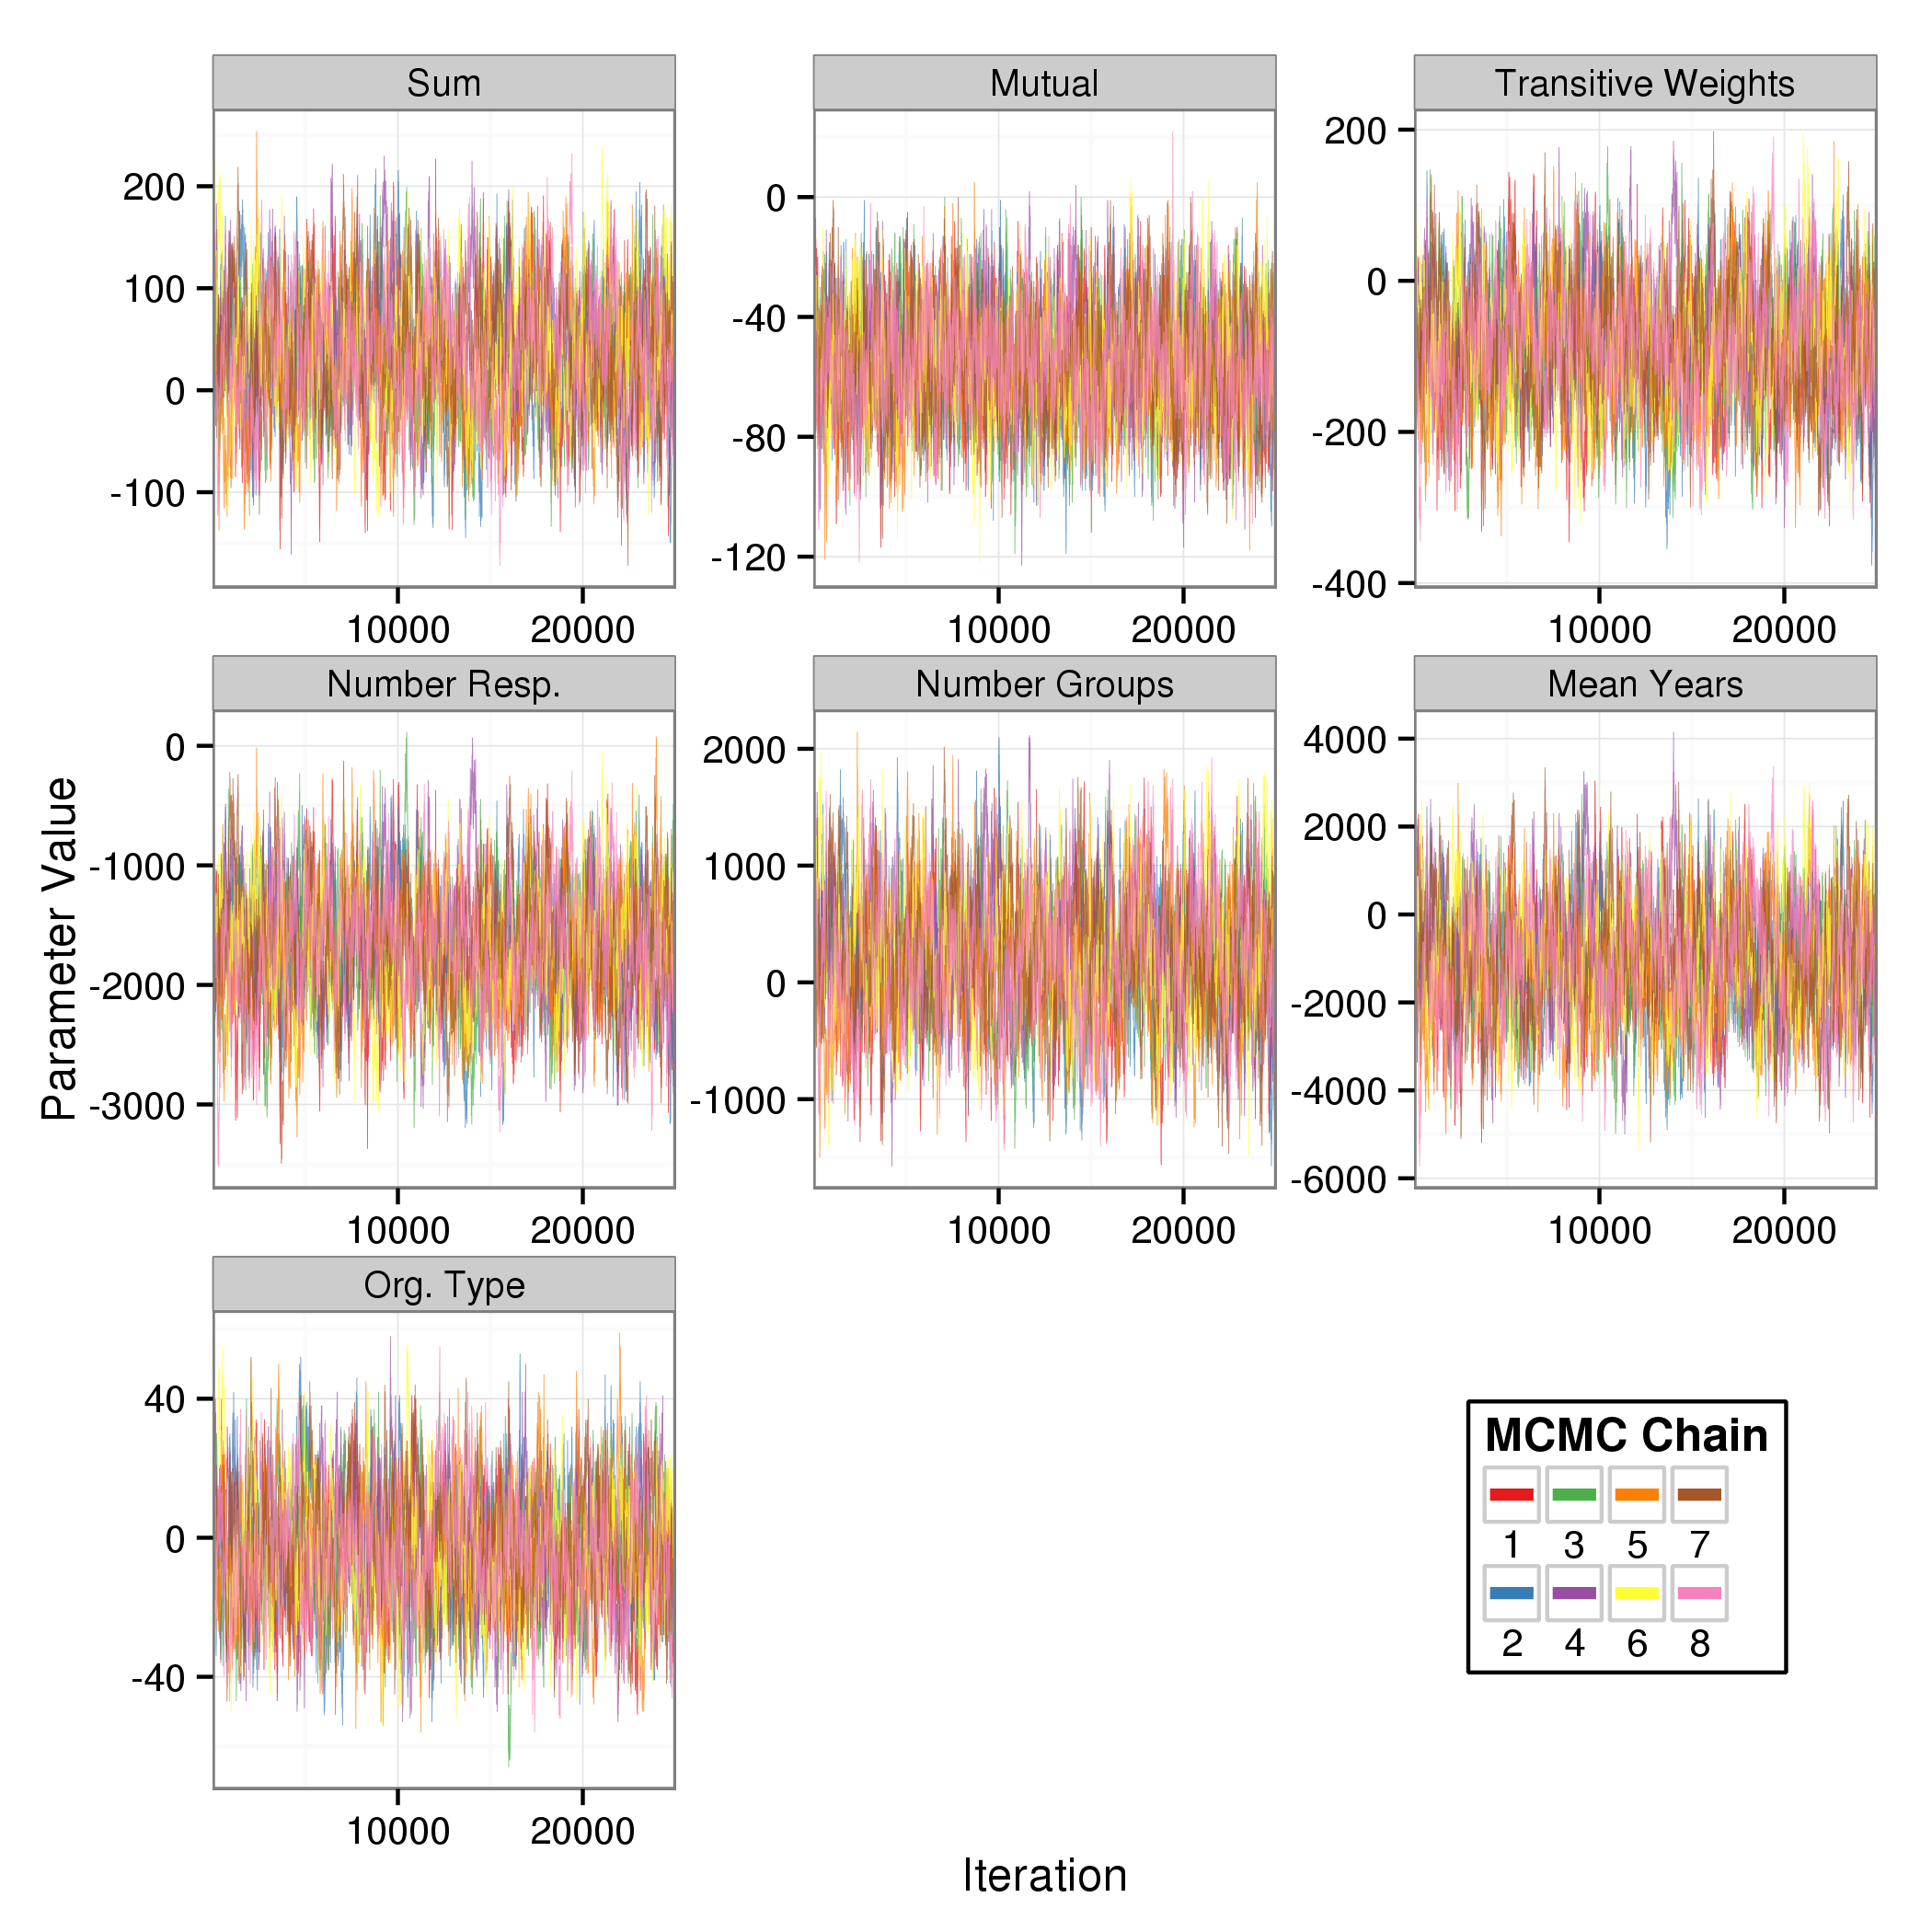
\includegraphics[width=6.5in]
{traceplotdu}
\label{figure:traceplots}
\end{figure}

Further, Figure \ref{figure:densityplots} shows smoothed parameter density plots from each MCMC run. As shown, in most cases each chain produces a unimodal distribution. The x-axis values in Figure \ref{figure:densityplots} represent the difference between the observed network statistics and the network statistics for each iteration of the MCMC routine. One can verify model convergence by seeing that the density plot for each parameter (normalized by the observed statistic) has a mean near zero and is normally distributed; in other words, the model has converged to the observed network. In this case, one observes that most distributions are centered closely to zero and appear to be roughly normally distributed. Most importantly, the overall mean in each case appears to be centered near zero as well, which demonstrates that the fitted model nicely approximates the observed data.

\begin{figure}[!ht]
\caption{\textit{Density Plots of MCMC Parameters}}
\graphicspath{ {`/Users/TScott/Google\space Drive/elwha/NetworkChapter'}}
\noindent
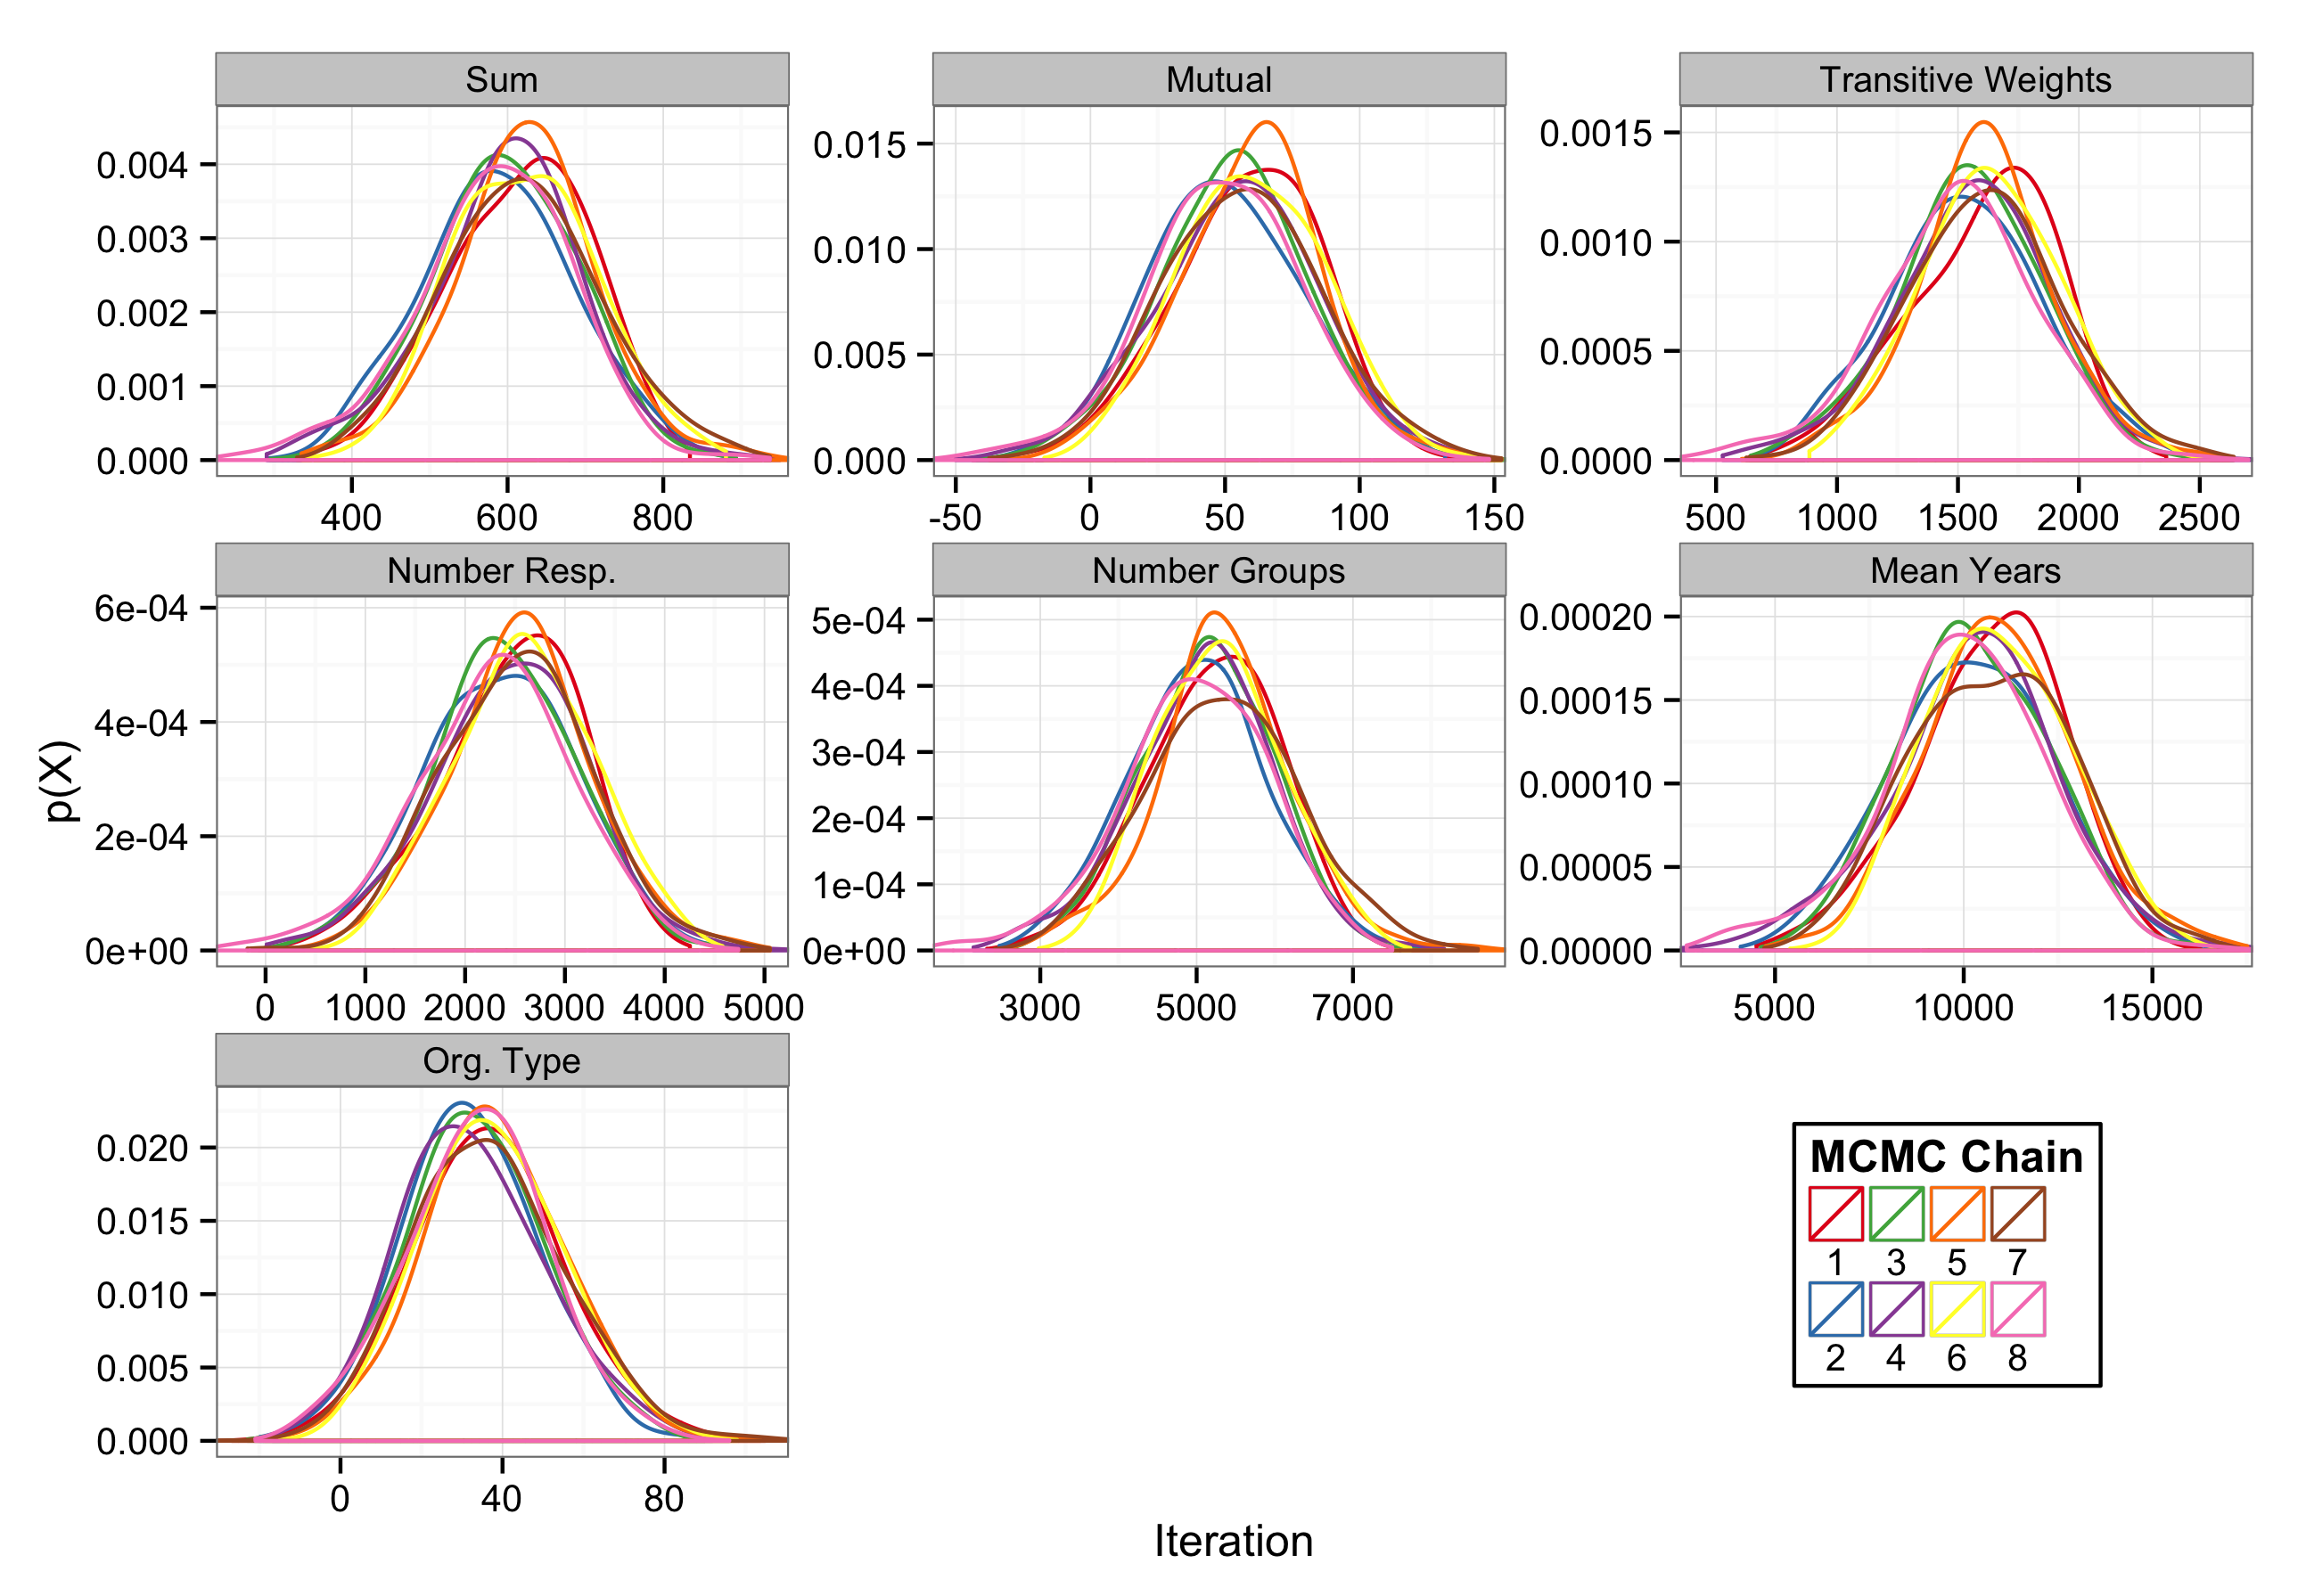
\includegraphics[width=6.5in]
{densityplotdu}
\label{figure:densityplots}
\end{figure}

\subsection{Baseline Models}

Having demonstrated that both models are a good fit for the observed data, I now proceed to analyze the baseline models. Table \ref{table:basemods} presents the restricted model, with only structural and actor-related covariates. Coefficients are interpreted as an additive effect on the natural log of the expected tie value (which can thus be exponentiated to produce a more easily interpretable multiplicative effect). The Sum parameter is a measure of network density, as it reflects the total sum of tie values observed in the network. For instance, a network with more joint implementation ties (each having a value of 3) will have a higher density than a network with more informal consultation ties (each having a value of 1). The strongly negative Sum parameters in Table \ref{table:basemods} show the network is very sparse. Specifically, the parameter can be exponentiated to show that the expected tie value between two randomly selected organizations is $0.015$ ($exp^{-4.18} = 0.015$). It is expected that these values are quite low, simply because most organizations in the network do not have any type of tie to most other organizations (with 221 organizations there are 48,620 potential ties).

%input table with base models: label = `table:basemods'

% Table created by stargazer v.5.1 by Marek Hlavac, Harvard University. E-mail: hlavac at fas.harvard.edu
% Date and time: Tue, Dec 09, 2014 - 10:20:25
\begin{table}[!htbp] \centering 
  \caption{Baseline Models} 
  \label{table:basemods} 
\begin{tabular}{@{\extracolsep{5pt}}lccc} 
\\[-1.8ex]\hline \\[-1.8ex] 
 & Baseline Model & Group Participation & Group Participation$^2$ \\ 
\hline \\[-1.8ex] 
 Sum & $-$4.19$^{***}$ & $-$4.19$^{***}$ & $-$4.44$^{***}$ \\ 
  & (0.06) & (0.06) & (0.07) \\ 
  Mutual & 1.70$^{***}$ & 1.65$^{***}$ & 1.60$^{***}$ \\ 
  & (0.09) & (0.09) & (0.08) \\ 
  Transitivity & 0.11$^{***}$ & 0.10$^{***}$ & 0.08$^{**}$ \\ 
  & (0.03) & (0.03) & (0.04) \\ 
  Num. Resp. & 0.16$^{***}$ & 0.12$^{***}$ & 0.07$^{***}$ \\ 
  & (0.005) & (0.01) & (0.01) \\ 
  Num.Groups & $-$0.01$^{**}$ & $-$0.01$^{*}$ & $-$0.01$^{***}$ \\ 
  & (0.01) & (0.005) & (0.01) \\ 
  Years & 0.01$^{***}$ & 0.01$^{***}$ & 0.01$^{***}$ \\ 
  & (0.002) & (0.002) & (0.002) \\ 
  Org. Type & 0.26$^{***}$ & 0.28$^{***}$ & 0.25$^{***}$ \\ 
  & (0.07) & (0.07) & (0.07) \\ 
  Group Partic. &  & 0.03$^{***}$ & 0.11$^{***}$ \\ 
  &  & (0.002) & (0.01) \\ 
  Group Partic.$^2$ &  &  & $-$0.002$^{***}$ \\ 
  &  &  & (0.0002) \\ 
 AIC & $-$115,800.10 & $-$115,928.30 & $-$116,144.70 \\ 
BIC & $-$115,738.60 & $-$115,858.00 & $-$116,065.60 \\ 
\hline \\[-1.8ex] 
\multicolumn{4}{l}{\textit{Note:} $^{***}$p $<$ .01; $^{**}$p $<$ .05; $^{*}$p $<$ .1} \\ 
\end{tabular} 
\end{table} 


Each of the remaining parameters acts multiplicatively on the sum term. The Mutual parameter\footnote{Which takes the general form $g_{\leftrightarrow} = \sum_{(i,j) \in Y} \min{( y_{(i,j)} y_{(j,i)})}$} represents the change in probability of observing a tie between two organizations, for instance a tie from A to B, given an observed tie from B to A. The observed values for “mutuality” in the data are taken to be the minimum value or count of the two reciprocal dyads ($min(y_{i,j},y_{j,i}$). As expected, this shows a strong and significant correlation between both the tie counts associated with a network dyad. In other words, I would expect A to be much more likely to report a tie to B given that B has already reported a tie to A (consider the informational jump in this case from the basic probability associated with two randomly selected organizations). The expected value of a tie from one organization to another increases by $417\%$ ($exp^{1.70} = 5.47$) for each tie observed in the opposite direction.

The Transitive Weights parameter\footnote{Which takes the general form $g(y) = \sum_{(i,j) \in Y} \min(y_{i,j},\max\limits_{k \in N}(\min(y_{i,k},y_{k,j})))$ in which the strength of a two-path from $i$ to $j$ is defined by the minimum value along said path, and the statistic then reflects the sum of minimum over the dyads ($i, j$) and the value of the strongest two-path in between each $i$ and $j$ combination.} is interpreted in a similar way as that of the Mutual parameter, but in this case refers to the degree to which presence and strength of a two-path\footnote{If there is an edge from A to C and from C to B, A and B are said to be connected via a two-path} between two organizations affects the expected value of a direct tie between the same two organizations. Table \ref{table:basemods} shows that for each unit by which the highest value two-path between two organizations increases in value (for instance, if $y_{i,j} = y_{j,k} = 2$ instead of $y_{i,j} = y_{j,k} = 1$), the expected tie value between the organizations increases by $11\%$ ($exp^{0.10} = 1.11$).

The baseline model also fits four node-specific variables that are predicted to affect the probability of observing ties associated with a given node. The Number of Respondents (Num. Resp.) parameter reflects the predicted impact on the expected value of a tie associated with an organization that has an additional respondent in the survey. This parameter should be positive, since having an additional respondent increases the number of ties that can possibly be reported by an organization. As expected, this parameter is significant and positive, predicting a $17\%$ ($exp^{0.16} = 1.17$) increase in the expected value of a tie between the focal organization and each other organization. Interestingly, the parameter reflecting the suggested effect of each additional group an organization participates in is statistically significant and negative; however, the magnitude of this suggested relationship is minimal (only a $1\%$ decrease in the probability of observing a tie between the focal organization and another organization [$exp^{-0.01} = 0.99$]). The `Years' parameter models the predicted association between the number of years a respondent has been at their position and the value of a network tie. This parameter is small, but positive, with each year predicting a 1\% increase in the value of a tie ($exp^{0.01} = 1.01$). Finally, the `Org. Type' variable compares the expected tie value to similar organizations. Specifically, organizations are coded as 15 different types of organizations, including state agencies, consulting firms, and tribes.\footnote{The full list includes: environmental NGOs, city governments, local advocacy groups, local commissions, special districts, county governments, local outreach and education organizations, consulting firms, regional advocacy groups, tribes, federal agencies, parks and reserves, natural resource extraction firms, universities and research organizations, regional commissions, and state agencies.} The predicted value of a tie (i.e., the strength of a collaborative tie) to a similar organization is 31\% greater than that of a dissimilar organization ($exp^{0.27} = 1.31$); this is consistent with the commonly observed network phenomenon of homophily, in which actors with common characteristics are more likely to be linked in a network \parencite{prell2012,kolaczyk2009}.

The second column of Table \ref{table:basemods} adds a generic collaborative group participation metric to the baseline model shown in column one. Simply being a member of a group does not necessarily speak to the degree to which an organization actually participates. One would expect that interorganizational transaction costs are reduced in proportion to the degree of participation, and further that the strength of the association between group membership and tie formation should be commensurate with the degree to which organizations actually participate in collaborative groups. In order to test this, group participation is measured in terms reported engagement in seven different group activities for each group in which a respondent reports membership: (1) send or respond to group emails; (2) attend group meetings; (3) attend other group events; (4) participate in group projects or programs; (5) read or review group reports and documents; (6) produce group reports or documents; and (7) other types of participation. This value is then divided by 7 to produce a fractional measure of participation in a given group. This per-group participation measure is then summed to produce an overall measure of group participation for a given organization. While this parameter is shown to be positive and significantly different from zero, it appears to be of limited practical significance: a one-unit increase in group participation increases the expected value of a tie involving the focal organization by $3\%$ ($exp^{0.03} = 1.03$). One likely reason for this is that this linear participation metric does not account for the fact that there are likely to be diminishing returns associated with a marginal increase in group membership and participation \parencite{lubell2010}. The third column shows a model with an additional quadratic term for group participation. In this model, the predicted linear association between group participation and tie occurence becomes much stronger, predicted a $12\%$ increase in expected tie value ($exp^{0.11} = 1.12$), and the quadratic term is very small but negative. In other words, participation in a collaborative group does strongly predict an increase in tie values associated with the participating organization, but this predicted increase diminishes as the number of groups the organization participates in increases.

\subsection{Controlling for Existing Groups}

%input tables for controlling for existing group models: label = `table:splitpart'

% Table created by stargazer v.4.5.3 by Marek Hlavac, Harvard University. E-mail: hlavac at fas.harvard.edu
% Date and time: Mon, Apr 14, 2014 - 16:20:29
\begin{table}[!htbp] \centering 
  \caption{Existing Groups} 
  \label{table:splitpart} 
\begin{tabular}{@{\extracolsep{5pt}}lccc} 
\\[-1.8ex]\hline \\[-1.8ex] 
 & Non-PSP & PSP + Non-PSP & PSP * Non-PSP \\ 
\hline \\[-1.8ex] 
 Group Partic. non-PSP & 0.02$^{***}$ & 0.02$^{***}$ & 0.15$^{***}$ \\ 
  & (0.003) & (0.003) & (0.01) \\ 
  Group Partic. PSP &  & 0.01 & 0.12$^{***}$ \\ 
  &  & (0.01) & (0.01) \\ 
  Group Partic. non-PSP*PSP &  &  & $-$0.03$^{***}$ \\ 
  &  &  & (0.001) \\ 
 AIC & $-$106,251.70 & $-$106,298.40 & $-$106,710.60 \\ 
BIC & $-$106,181.40 & $-$106,219.30 & $-$106,622.70 \\ 
\hline \\[-1.8ex] 
\textit{Note:} & \multicolumn{3}{l}{$^{***}$p $<$ .01; $^{**}$p $<$ .05; $^{*}$p $<$ .1} \\ 
\normalsize 
\end{tabular} 
\end{table} 


The issue of diminishing marginal returns is critical to gauging the effectiveness of a network intervention. Given that numerous collaborative groups were already in existence there is a very real potential for redundancy. As described above, recent policy literature discussing how organizations operate within complex institutional environments \parencite[see][]{lubell2013}, along with empirical findings regarding the practical limitations most managers and officials face \parencite{thomas2003,margerum2011}. Simply put, organizations have a limited capacity for collaborative activities \parencite{lubell2010}. Thus, a government-sponsored collaborative group intended to further enhance network coordination might actually motivate organizations to reallocate their existing efforts across these multiple arenas without a net increase. Whereas the quadratic term in Table \ref{table:basemods} tests this phenomenon generally (by examining overall participation in Puget Sound area collaborative groups regardless of origin), I examine the PSP's intervention specifically by dividing the Group Participation variable into two categories: participation in non-PSP affiliated groups (i.e., those in existence prior to the network intervention) and participation in PSP sponsored groups. Table \ref{table:splitpart} shows the results for three models, fitting: participation in only non-PSP groups, participation in both group types, and a term interacting participation in each group type (the base parameters are omitted in these and subsequent tables, but are included in all models). What is observed in the unrestricted model (column three) is that participation in either type of group is positively associated with the expected value of an interorganizational tie, but that there are diminishing returns to participation in both types of groups. In other words, the association between group participation and the expected value of a network tie diminishes to the extent that the organizations involved in PSP-sponsored groups already participated in non-PSP groups. This indicates that the PSP's network intervention had the greatest impact on organizations that were not already heavily involved in collaborative groups. Pragmatically, this makes a great deal of sense; organizations more heavily involved in collaborative groups prior to the network intervention presumably already had greater opportunity to engage and initiative ties with other organizations.

\subsection{Potential Confounding}

Obviously, one cannot simply look at the above results and conclude that the PSP's intervention was successful (or unsuccessful) in terms of motivating increased interorganizational collaboration. As discussed in above section above, it is possible that group participation and interorganizational collaboration are both products of unobserved organizational characteristics such as motivation to engage with other organizations. There are certainly organizations for whom participation in collaborative groups and direct collaboration with other organizations is more beneficial, and organizations for whom both of these activities are less beneficial. What I seek to examine in this analysis, however, is whether there is an observable impact of government-sponsored collaborative groups net of these inherent characteristics. In other words, regardless of natural “collaborative proclivity,” does the the likelihood of observing interorganizational collaboration change in association with a marginal change in collaborative group participation? Using a series of model specifications, this relationship is triangulated using a series of progressively more strict coding schemes and comparing the coefficients.

%input tables for triangulating participations: label = `table:partmods'

% Table created by stargazer v.5.1 by Marek Hlavac, Harvard University. E-mail: hlavac at fas.harvard.edu
% Date and time: Thu, Apr 16, 2015 - 04:29:52 PM
\begin{table}[!htbp] \centering 
  \caption{Triangulating Participation} 
  \label{table:partmods} 
\begin{tabular}{@{\extracolsep{5pt}}lccc} 
\\[-1.8ex]\hline \\[-1.8ex] 
 & Group Participation & Direct Participation & Co-Participation \\ 
\hline \\[-1.8ex] 
 Group Partic. non-PSP & 0.04$^{***}$ &  &  \\ 
  & (0.01) &  &  \\ 
  Group Partic. PSP & 0.03$^{***}$ &  &  \\ 
  & (0.01) &  &  \\ 
  Group Partic. non-PSP*PSP & $-$0.01$^{***}$ &  &  \\ 
  & (0.001) &  &  \\ 
  edgecov.dpn7.sum &  & 0.46$^{***}$ &  \\ 
  &  & (0.02) &  \\ 
  edgecov.dppsp7.sum &  & 0.76$^{***}$ &  \\ 
  &  & (0.03) &  \\ 
  edgecov.dpx7.sum &  & $-$0.03$^{***}$ &  \\ 
  &  & (0.002) &  \\ 
  edgecov.spn7.sum &  &  & 0.94$^{***}$ \\ 
  &  &  & (0.04) \\ 
  edgecov.sppsp7.sum &  &  & 1.37$^{***}$ \\ 
  &  &  & (0.06) \\ 
  edgecov.spx7.sum &  &  & $-$0.09$^{***}$ \\ 
  &  &  & (0.01) \\ 
 AIC & 56,313.17 & $-$106,794.40 & $-$110,112.40 \\ 
BIC & 56,401.09 & $-$106,706.50 & $-$110,024.50 \\ 
\hline \\[-1.8ex] 
\textit{Note:} & \multicolumn{3}{l}{$^{***}$p $<$ .01; $^{**}$p $<$ .05; $^{*}$p $<$ .1} \\ 
\end{tabular} 
\end{table} 


Table \ref{table:partmods} shows the results of three models, the first the same model as found in the the third column of Table \ref{table:splitpart} and the next two representing increasingly stringent ways of coding for group participation. If participation in collaborative groups is a driver of interorganizational networking, then the impact of a collaborative group should primarily be experienced with regards to organizations that are actually members of the same group. In other words, while collaborative groups might certainly increase awareness of and access even to other organizations that are not in the same group, it stands to reason that the association between participation and network ties should be concentrated amongst organizations who actually are members of the same group. Thus, I create a ‘’Direct Participation’’ measure, by conditioning total participation on group membership. Each organization is given a distinct Direct Participation score to every other organization. This score is zero if the organizations do not share a group. If two organizations do share at least one group, then the Direct Participation score from Organization A to Organization B reflects group participation reported by Organization A within groups of which Organization B is also a member. If group participation and interorganizational networking are confounded by a common cause, then the predicted association between the general metric `'Group Participation'' and the occurrence of network ties (column one) should not be meaningfully different than the predicted association between “Direct Participation” and the occurrence of network ties (column two). However, what I observe in Table \ref{table:partmods} is that the coefficients become much stronger. A one unit increase in general Group Participation in a PSP-affiliated group increases the predicted value of a network tie by $13\%$ ($exp^{0.12} = 0.13$), whereas as one unit increase in Direct Participation in a PSP-affiliated group increase the predicted value of a network tie by $138\%$ ($exp^{0.87} = 2.38$).

While Direct Participation focuses on organizations that actually share group membership, the theoretical mechanisms by which collaborative groups are hypothesized to reduce transaction costs (and thus engender increased interorganizational collaboration) holds that collaboration is motivated by ‘’principled engagement’’ and ‘’increased capacity for joint action’’ \parencite{emerson2012}. In other words, by engaging directly with one another, organizations build trust and learn more about one another’s needs, interests, and capabilities, thereby decreasing the costs associated with searching for, initiating, and maintaining network ties. Practically speaking, this can only occur if both organizations “show up” and actually encounter one another in group activities. Thus, I code a third metric, ‘’Co-Participation,’’ in which the covariate associated with each possible pair of organizations is the minimum combined Direct Participation measure shared by the two organizations (column three). For instance, if Organization A and Organization B are both members of one group, in which A participates in five of seven activities and B participates in three of seven, then the Co-Participation score for dyad AB (and for dyad BA) is three.\footnote{Note that I purposefully do not match on specific activities, as doing so would inject a great deal of false specificity into the model. For instance, when two organizations both report that they participate in group events or help write group documents, there is no way to verify whether these organizations participated in the same events or have helped write the same documents. Accordingly, I take the conservative approach of not matching on specific activities; this approach is conservative because if collaborative ties are in fact strongly associated with participation in the same group activities, then the strength of this association will be underestimated in my model.} The coefficients in column three of Table \ref{table:partmods} are even stronger than those in column two. A one unit increase in Co-Participation increases the predicted value of a network tie by $395\%$ ($exp^{1.60} = 4.95$). While this is by no means conclusive evidence about the causal effect of sponsoring collaborative management groups, these results are what one would expect to observe if providing increased opportunities for organizations to engage with one another does in fact engender increased interorganizational collaboration. Realistically, it is likely both that this occurs and that counfounding is present.

\subsection{Reverse Causality}

%input tables for triangulating participations: label = `table:pastties'

% Table created by stargazer v.5.1 by Marek Hlavac, Harvard University. E-mail: hlavac at fas.harvard.edu
% Date and time: Mon, May 18, 2015 - 09:40:52 AM
\begin{table}[!htbp] \centering 
  \caption{Pre-Existing Ties} 
  \label{table:pastties} 
\begin{tabular}{@{\extracolsep{5pt}}lc} 
\\[-1.8ex]\hline \\[-1.8ex] 
 & Past Tie \\ 
\hline \\[-1.8ex] 
 Past Tie (PT) & 4.73$^{***}$ \\ 
  & (0.07) \\ 
  All Group Co-Part. & 1.65$^{***}$ \\ 
  & (0.06) \\ 
  All Group Co-Part.$^2$ & $-$0.20$^{***}$ \\ 
  & (0.01) \\ 
  All Group Co-Part. * PT & $-$0.88$^{***}$ \\ 
  & (0.05) \\ 
 AIC & $-$125,240.50 \\ 
BIC & $-$125,143.80 \\ 
\hline \\[-1.8ex] 
\textit{Note:} & \multicolumn{1}{l}{$^{***}$p $<$ .01; $^{**}$p $<$ .05; $^{*}$p $<$ .1} \\ 
\end{tabular} 
\end{table} 


One potential contributor to the overall magnitude of the Direct Participation and Co-Participation parameters is the combined sparsity of the overall network and the informational value these parameters provide about the network proximity of any two organizations. Specifically, it is plausible that instead of forming relationships within collaborative groups, organizations invite other organizations with whom they already engage to participate in groups. This would be reverse causality, in which network relationships drive collaborative group participation, rather than the other way around.

In order to test this, the survey instrument asked each respondent to report whether each reported interorganizational tie had existed prior to the PSP’s network intervention (i.e., more than five years ago). This provides a rough approximation as to whether a network tie predates the intervention (the exception being in cases where the tie was initiated within the last five years, but prior to the organization becoming a group member). While this does not provide as robust a picture as would a true longitudinal analysis, it does provide a general gauge of the extent to which reverse causality might be at play by comparing how the association between group participation and interorganizational ties differs between ties that existed prior to the PSP’s intervention and those that did not.

Table \ref{table:pastties} presents results from a model that includes all of the covariates specified in the baseline model and four additional parameters. First, the model fits a binary term for each potential dyad (pair of organizations) that reflects whether the tie reported from Organization A to Organization B was reported to exist prior to the PSP's network intervention. For a binary network, it would not be feasible to use this metric, since the metric would be a perfect predictor of the affirmative presence of a tie (but not tie absence, since more newly formed ties are reported as well)\footnote{Of the 1045 ties observed in the data, 581 are reported to be ties that pre-date the network intervention.}. However, since this analysis models valued network ties, it can examine how the fact that a tie was also reported to exist before the network intervention impacts the expected value of the tie after the intervention.\footnote{Further, given the self-reinforcing nature of network relations \parencite{ostrom2000, putnam2000}, one might also expect that on average, ties that existed five years ago should be stronger than ties that did not. For instance, if an informal consultation tie is reported to have existed five years ago between two organizations, then there should be a stronger probability of observing a coordinated planning or joint implementation tie between these two organizations relative to two randomly selected organizations.} As should be expected, this parameter is positive and very strong in magnitude; this result is not substantively interesting, however, since past ties reported in the survey instrument are restricted to currently existing ties. Table \ref{table:pastties} then fits both a linear and a quadratic term for Co-Participation in both PSP and non-PSP groups. This metric is calculated in the exact same way as the metrics in column three of Table \ref{table:partmods}, but in this case combines participation in both types of group. As in Table \ref{table:partmods}, the linear parameter is positive and strong in magnitude, and the quadratic parameter is negative, again demonstrating a diminishing marginal predicted association.

The parameter of interest in Table \ref{table:pastties} is the fourth parameter, an interaction term between co-participation in collaborative groups and the fact that a tie was reported to have existed prior to the PSP's network intervention. This parameter is negative and large in magnitude; that a tie of any value existed prior to the network intervention decreases the association between co-participation in a collaborative group and the value of a network tie by $69\%$ ($exp^{-0.89} = 0.41$). In other words, reverse causality appears to be of issue. Note however that the strong positive relationship between co-participation and tie value amongst organizations that did not have a tie prior to the network intervention remains. Thus, as with the issue of confounding examined above, it is likely that the relationship works in both ways: organizations that share network ties are likely to then join and participate in the same collaborative groups, and organizations that join and participate in the same collaborative group are likely to then initiate a direct network tie.

\section{Discussion/Conclusion}

These results provide empirical evidence as to how government intervention in a policy network is associated with changes in network structure and function. Theory indicates that interorganizational collaborative groups facilitate network relationships by providing a forum for organizations to engage with one another and learn more about the goals and capabilities of organizations within the network \parencite{emerson2012}. Repeated interactions and joint activities reduce interorganizational transaction costs by fostering trust and cooperative norms \parencite{ostrom2000} and social capital \parencite{putnam2000}. Many analyses of collaborative groups and organizational networks treat such factors as a given. From a policymakers’ perspective, however, what is of primary interest--and what is largely unaddressed in the literature--is how government can intervene to change an organizational network if desired. The justification for public funds and resources devoted to collaborative management groups is typically providing a forum and mechanisms for interorganizational engagement will in turn engender increased coordination and cooperation within an organizational network, but these claims have yet to be systematically evaluated.

Accordingly, this analysis builds on the work of \textcite{schneider2003}, who demonstrate the overall change in network conditions associated with a network intervention by government actors (e.g., denser networks), and \textcite{henry2011}, who model the role of social capital as a driver of policy network structure, by examining the relationship between government network interventions and the network behavior of individual organizations. This relationship is indirect, because a network intervention can alter the incentive structure individual organizations face, but does not directly address the goals, beliefs, and motivations of network organizations. Thus, the extent to which government can motivate interorganizational collaboration amongst independent actors is an open question.

This analysis finds a strong positive association between participation in collaborative groups and the number--and intensity-- of interorganizational ties an organization has. Thus, it complements the findings of CITATION REDACTED, which examines the specific mechanisms by which collaborative groups are hypothesized to reduce the transaction costs organizations face with regards to networking (and thus motivate the formation and maintenance of network ties). Further, modeling the comparative intensity of an interorganizational relationship (consultation, planning, or implementation), this analysis is able to model this relationship in a more nuanced fashion than does the policy network literature which uses binary ERGMs (e.g., CITATION REDACTED, \cite{lubell2012, gerber2013, schneider2003}).

While these results suggest that government-sponsored collaborative groups enhance interorganizational networks, there are several very important considerations that also emerge in this regard. First, as demonstrated by \textcite{lubell2010, lubell2011-a}, organizations are faced with numerous networking opportunities and are limited in their ability to engage in collaborative groups and to maintain ties with individual organizations. In keeping with this, I identify a diminishing relationship between group participation and interorganizational collaboration as the number of groups an organization participates in increases. Particularly, this analysis suggests that a network intervention has a lessened effect on organizations that already participate in other collaborative groups. This indicates that interventions should be targeted towards organizations that are not already involved in other groups.

I also (unsurprisingly) find evidence that collaborative groups are subject to selection bias; namely, that organizations that are more willing to participate in collaborative groups tend to also be more willing to engage in direct collaboration with other organizations. While these observational data cannot eliminate the role of selection bias, by modeling increasingly strict conceptions of group participation, I am able to establish that the predicted relationship between group participation and the level of interorganizational collaboration is strongest among organizations that both participate to a similar extent in the same group(s). This suggests that the collaborative group itself has some role in driving network structure, net of intrinsic organizational characteristics.

Finally, I find strong evidence that collaborative group participation is in part driven by pre-existing network relationships, and that this predicted relationship largely mitigates the predicted relationship between participation and the value of a network tie. This is critical for the design and implementation of network interventions such as collaborative groups, because it indicates that little network change should be expected if a network intervention simply involves already linked actors. However, these results also demonstrate an opportunity for policy makers to enhance an existing network by taking care to craft groups that are not highly redundant and taking efforts to involve peripheral organizations in the network.

In order to move forward on better understanding these issues, longitudinal network data are a critical need. While it can be expensive and difficult to collect repeated measures network data (even in collecting these cross-sectional data, the author encountered many practitioners who were too busy to participate and had too many competing demands on their time), a longitudinal perspective is required to better understand network dynamics over time and trace the long-term impact of public policy interventions. While it is clear that governments are beginning to intervene to address perceived network failures just as they seek to remedy market failures and other institutional shortcomings, there is not yet a large body of knowledge built up surrounding the use of various policy tools for network interventions. This analysis contributes to this evidence base with the goal of helping policy makers to fashion context-appropriate, customized interventions that can effectively address network coordination issues.

\nocite{handcock2014-a,analytics2014,butts2014}

\printbibliography

\end{document}

































